\documentclass[11pt]{article}
\usepackage[margin=0.8in]{geometry}
\usepackage[T1]{fontenc}
\usepackage{lmodern}
\usepackage{microtype}
\usepackage{amssymb}
\usepackage{booktabs}
\usepackage{longtable}
\usepackage{xcolor}
\usepackage{listings}
\usepackage{graphicx}
\usepackage{pdflscape}
\usepackage{hyperref}
\usepackage{enumitem}
\hypersetup{colorlinks=true,linkcolor=blue!55!black,urlcolor=blue!55!black}
\lstset{basicstyle=\ttfamily\small,breaklines=true,frame=single,rulecolor=\color{black!20},columns=fullflexible,keepspaces=true}
\lstdefinestyle{python}{
  language=Python,
  morekeywords={True,False,None},
  basicstyle=\ttfamily\small,
  keywordstyle=\color{blue!75!black}\bfseries,
  emph={reduce,assign,field,choose,constant,arg,record,put,map_items,Machine,Command,StateType,QuestionFreeText,QuestionNumerical,Survey,SharedStateMap,InterviewSchedule,current,states},
  emphstyle=\color{violet!75!black}\bfseries,
  commentstyle=\color{green!40!black}\itshape,
  stringstyle=\color{red!65!black},
  numberstyle=\color{orange!75!black},
  showstringspaces=false,
  breaklines=true,
  frame=single,
  rulecolor=\color{black!20},
  columns=fullflexible,
  keepspaces=true
}
\setlist{nosep,leftmargin=*}
\title{A Shared-State EDSL Port of the SPSB-IPV Auction}
\author{Implementation and results analysis}
\date{October 9, 2026}

\begin{document}
\maketitle

\begin{abstract}
This note gives a formal and implementation-level account of a shared-state EDSL implementation of a three-bidder, one-round sealed-bid second-price auction with independent private values (SPSB-IPV). It specifies the machine state and transitions, follows one auction from scope creation through finalization, and analyzes 100 auctions (300 bidders). The split plan/bid prompt differs from the archived one-response treatment, so these results describe a new EDSL treatment rather than a direct reproduction of the published cell.
\end{abstract}

\section{Auction specification and machine definition}

The port implements the source cell \texttt{configs/experiments/01\_01\_spsb\_ipv.yaml}: one sealed-bid, second-price auction with three bidders, one round, and independent private values from 0 through 49. The bid increment is \$0.1. The EDSL machine, survey, and run builder are in \texttt{edsl\_replication/spsb\_ipv\_shared\_state.py}. The machine owns the auction state and settlement rule; Python constructs agents and prompts and invokes the EDSL runner.

\section{Formal state model and settlement}

The implementation follows the new EDSL separation between a machine definition, a shared-state definition, a scoped state handle, and an execution backend. The machine is a serializable description of fields, commands, expressions, views, and completion effects. It contains no Python auction callback and no database connection.

\subsection{Fields and command}

The \texttt{SPSB\_IPV} machine has one named constant, \texttt{bidder\_count=3}, and these state fields:

\begin{longtable}{p{0.20\linewidth}p{0.70\linewidth}}
\toprule
Field & Meaning \\
\midrule
\endhead
\texttt{bids} & Map keyed by bidder ID. Each entry stores bidder ID, seat, private value, and submitted amount. \\
\texttt{winner} & Bidder ID selected at close. \\
\texttt{winning\_bid} & Highest submitted amount. \\
\texttt{price} & Second-highest submitted amount. \\
\texttt{utilities} & Winner's value less price; zero for other bidders. \\
\bottomrule
\end{longtable}

\subsection{Mathematical definition of the machine}

Let the bidder set be $I=\{0,1,\ldots,N-1\}$, with $N=3$, and let $A=\{a_i:i\in I\}$ be the bidder identities. Each bidder $i$ has a fixed identity $a_i$, seat $s_i\in I$, private value $v_i\in\{0,\ldots,49\}$, and submitted bid $b_i\geq 0$. The active state for one auction scope is
\[
  x=(B,w,h,p,U), \qquad B:A\rightharpoonup (a_i,s_i,v_i,b_i),
\]
where $B$ is a partial map of received bids, $w$ is the winner, $h$ is the winning bid, $p$ is the price, and $U$ is the utility map. Initially, $B=\varnothing$, $w=h=p=\bot$, and $U=\varnothing$. The state is open until the completion predicate is true.

For an open state, the command \texttt{submit\_bid}$(a,s,v,b)$ performs the transition
\[
  \delta_{\mathrm{bid}}(x;a,s,v,b)
  = (B[a\mapsto(a,s,v,b)],w,h,p,U).
\]
In the implementation, $a$ is the map key, and the typed command requires text $a$, integer $s\geq0$, and numbers $v,b\geq0$. The intended protocol invokes this command once for each registered bidder.

Completion is the predicate
\[
  C(x)\iff |B|=N.
\]
When $C(x)$ first holds, let $\pi(B)$ sort the stored records by descending bid and then ascending seat. Write $r_1=\pi(B)_1$ and $r_2=\pi(B)_2$. The close transition sets
\[
  w=r_1.a,\qquad h=r_1.b,\qquad p=r_2.b,
\]
and, for each registered bidder $i$,
\[
  U(a_i)=\mathbf{1}[a_i=w]\,(v_i-p).
\]
Thus the winning bidder pays the second-highest submitted bid and every losing bidder receives zero utility. If highest bids tie, the lower seat wins because seat is the secondary sort key. This is a deterministic implementation choice; the legacy simulator randomly selects among tied highest bidders.

The public view is a function of state and closed status $c$. It always returns $N$ and $|B|$. When $c=0$, it returns an empty bid map and null settlement fields; when $c=1$, it returns submitted amounts and $(w,h,p,U)$. Private values are not in the public view. The EDSL schedule uses a round-start snapshot for all reads, so each bidder observes the same pre-bid view even when interviews execute concurrently.

\noindent\textit{Core of \texttt{build\_machine}: the returned \texttt{Machine(...)} is the complete serialized mechanism definition.}
\begin{lstlisting}[style=python]
def build_machine(*, bidder_count: int) -> Machine:
    ranked = reduce(
        "sort_records", field("bids").values(),
        fields=("amount", "seat"), descending=(True, False),
    )
    winner = ranked.first()
    winner_id = winner.get("bidder")
    second_bid = choose(ranked.length() > 1, ranked.at(1).get("amount"), 0)
    utilities = map_items(
        field("bids"), key="bidder", value="bid",
        key_expr=local("bidder"),
        value_expr=(
            choose(local("bidder") == winner_id, local("bid").get("value"), 0)
            - choose(local("bidder") == winner_id, second_bid, 0)
        ),
    )
    return Machine(
        name="SPSB_IPV",
        constants={"bidder_count": bidder_count},
        fields={
            "bids": state_field(StateType.map(), {}),
            "winner": state_field(StateType.optional(StateType.text()), None),
            "winning_bid": state_field(StateType.optional(StateType.number()), None),
            "price": state_field(StateType.optional(StateType.number()), None),
            "utilities": state_field(StateType.map(), {}),
        },
        commands={
            "submit_bid": Command(
                inputs={
                    "bidder": StateType.text(),
                    "seat": StateType.integer(minimum=0),
                    "private_value": StateType.number(minimum=0),
                    "amount": StateType.number(minimum=0),
                },
                effects=(put("bids", arg("bidder"), record(
                    bidder=arg("bidder"), seat=arg("seat"),
                    value=arg("private_value"), amount=arg("amount"),
                )),),
            ),
        },
        view={
            "bidder_count": constant("bidder_count"),
            "bid_count": field("bids").length(),
            "bids": choose(current("closed"), map_items(
                field("bids"), key="bidder", value="bid",
                key_expr=local("bidder"),
                value_expr=local("bid").get("amount"),
            ), {}),
            "winner": choose(current("closed"), field("winner"), None),
            "winning_bid": choose(current("closed"), field("winning_bid"), None),
            "price": choose(current("closed"), field("price"), None),
            "utilities": choose(current("closed"), field("utilities"), {}),
        },
        complete_when=field("bids").length() == constant("bidder_count"),
        close_effects=(
            assign("winner", winner_id),
            assign("winning_bid", winner.get("amount")),
            assign("price", second_bid),
            assign("utilities", utilities),
        ),
    )
\end{lstlisting}

\subsection{Public view and sealed bids}

The machine view always exposes the fixed bidder count and the current bid count. It exposes bid amounts and settlement fields only when the state is closed. Before close, the view returns an empty bids map and null outcome values. Private values are never included in the public view. This gives the state definition an explicit information boundary rather than relying on prompt wording to hide bids.

The survey explicitly reads the auction state before the plan question. For every auction group, the schedule pins a snapshot at the beginning of the round. All three interviews therefore read the same pre-bid state, even if one inference call returns earlier than another. The snapshot policy is the mechanism that preserves simultaneous sealed bidding; worker concurrency alone would not guarantee it.

\subsection{Completion and close effects}

The machine completion expression is \texttt{bids.length() == bidder\_count}. The schedule supplies that typed completion condition as \texttt{finalize\_when}. Once the final distinct bid has been written, EDSL closes the machine and evaluates its declarative close effects:

\begin{enumerate}
  \item Sort bid records by amount descending and seat ascending.
  \item Select the first record as the winner and store its amount as the winning bid.
  \item Store the second record's amount as the price.
  \item Set winner utility to private value minus price; set all other bidder utilities to zero.
\end{enumerate}

Because the sort uses seat as the secondary key, ties resolve deterministically in favor of the lower seat. The legacy simulator selects randomly among tied highest bids. That difference matters for a faithful protocol replication, even if ties are uncommon in a particular sample.

\subsection{Machine diagram generated by EDSL}

The current EDSL checkout provides \texttt{Machine.show\_diagram()}. I used its \texttt{pydot} renderer on the same \texttt{SPSB\_IPV} machine defined above. The diagram lays out persistent fields, the \texttt{submit\_bid} command and its typed inputs/effects, the read-only view, and the completion/close lifecycle. Green edges mark writes, purple edges show view projections, and dashed edges mark state reads. The long lifecycle expressions make this a wide overview; the equations and Python definition above give their readable form. The full-resolution rendered image is also saved under \texttt{writeup/figures/} for zooming.

\clearpage
\begin{landscape}
\thispagestyle{plain}
\begin{center}
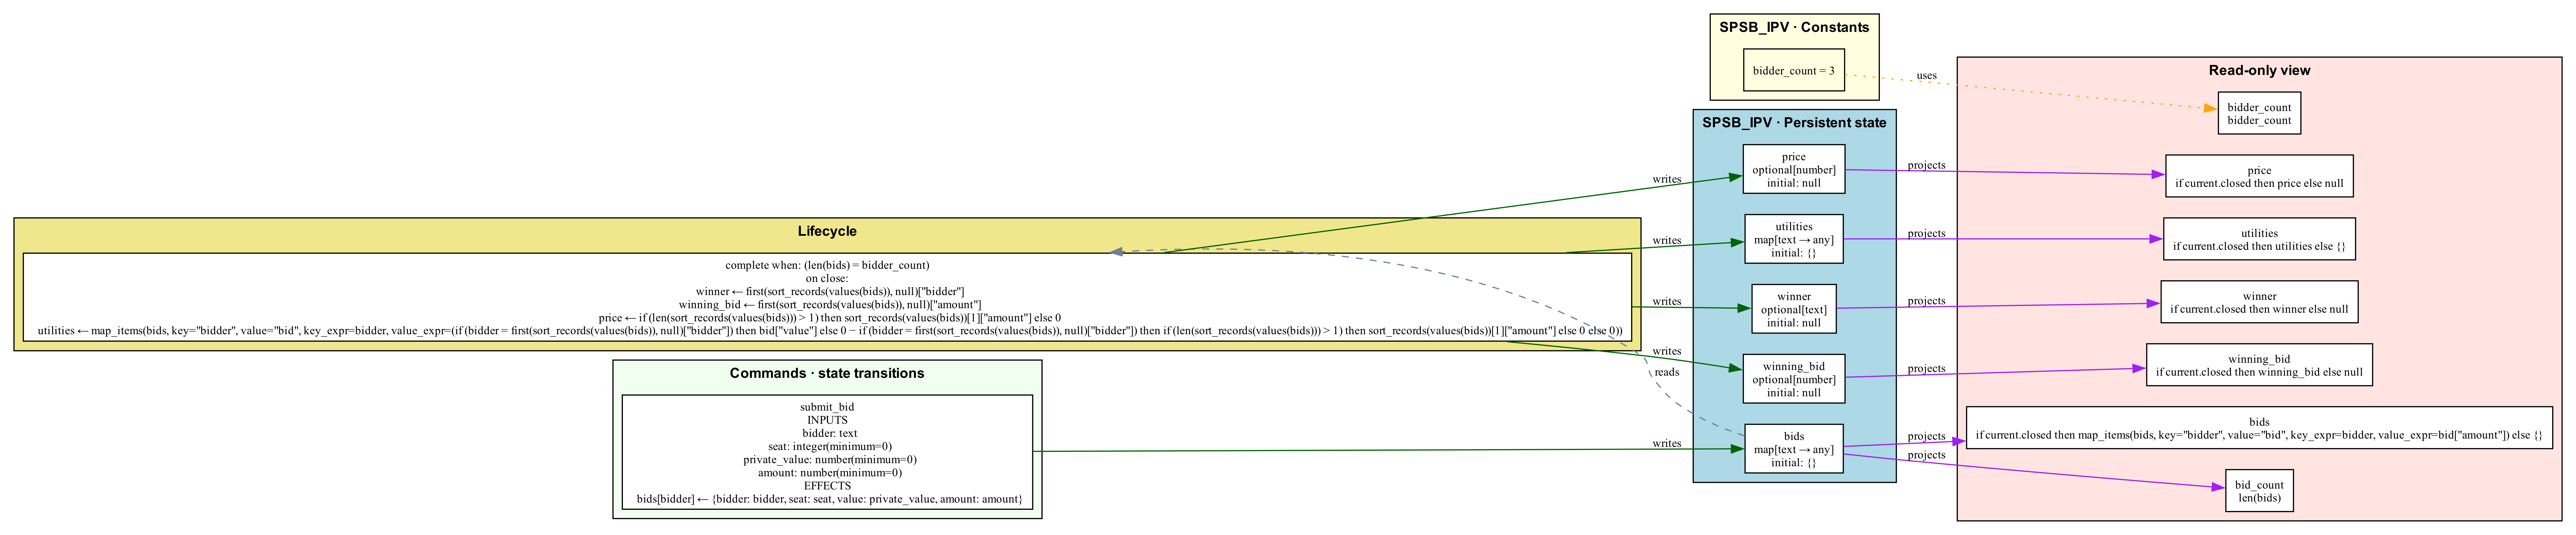
\includegraphics[width=0.98\linewidth]{figures/spsb_ipv_shared_state_machine.png}
\end{center}
\vspace{0.1in}
\noindent\textbf{Figure: EDSL machine visualization.} Generated by \texttt{Machine.show\_diagram(renderer="pydot", dpi=300)} from the auction machine. The edges connect declared state to the command, lifecycle, and read-only projection.
\end{landscape}
\clearpage

\section{Survey and routing}

\subsection{One job, many isolated auctions}

For \(R\) repetitions and three bidders, the builder creates \(3R\) EDSL agents in one job. Each agent carries \texttt{auction\_id}, bidder ID, seat, value, seed, and prompt text as traits. A single \texttt{SharedStateMap} contains the machine definition; its per-interview scope is \texttt{auction\_id}. The resulting data layout is:

\noindent\textit{Scope-to-state layout (schematic; not Python code).}
\begin{lstlisting}
SharedStateMap(state_id=one_run_id)
  auction-0000 -> SPSB_IPV state
  auction-0001 -> SPSB_IPV state
  ...
  auction-(R-1) -> SPSB_IPV state
\end{lstlisting}

The shared map's state ID is unique for each run. Scope keys distinguish auctions inside that run, so bidders in one auction share a state while different repetitions do not. This avoids creating a separate survey job and backend for every repetition.

\subsection{Answer-linked writes}

The survey sequence is a state read, a plan question, a numerical bid question, and a \texttt{submit\_bid} command. The command input \texttt{amount=bid.answer} is an answer reference, not an eagerly evaluated value. EDSL resolves it in the interview context after the numerical answer is accepted. Bidder, seat, and value are similarly read from the current agent's traits. The machine command is thus connected to a validated survey answer, while the state transition itself remains defined in the machine.

\subsection{Schedule semantics}

The run uses one concurrent snapshot round, grouped by auction ID. In the runner, round groups create dependency barriers between different rounds; with one round, the three bidder interviews in each auction group have no order dependencies. Before renderers start, the runner pins the group's shared-state checkpoint. When a read is executed under snapshot visibility, the backend renders the view at that checkpoint. Writes occur after answer commitment and are serialized by the backend transaction. The completion check and close transition can therefore happen only after the final accepted bid exists.

This schedule makes an important experimental claim explicit: bidder prompts are generated from the same empty auction state, so no bidder sees a rival's earlier bid or bid count progression. A serial schedule would define a different information treatment.

\subsection{Lifecycle of one auction and its interviews}

Each of the 100 repetitions is one independent scope, keyed by \texttt{auction\_id}; each scope receives three bidder interviews. The lifecycle below describes one such scope. The same shared-state definition is reused across all scopes, while each scope has its own state and event sequence.

\begin{enumerate}
  \item \textbf{Prepare the scope.} The builder draws three private values from the repetition's seed, creates three agents with bidder identity, seat, value, and rendered prompt traits, and assigns them a common \texttt{auction\_id}. The schedule groups those interviews under that key.
  \item \textbf{Pin the read view.} At the start of the concurrent round, the runner pins the shared-state snapshot for the group. Each interview executes \texttt{scoped.read()} before any model question. Since the scope is initially empty, the view reports three bidders and zero submitted bids, with no bid amounts or outcome exposed.
  \item \textbf{Elicit a plan and bid.} The model answers a free-text plan question, then a numerical bid question whose text includes that plan. The second response is constrained to be nonnegative. This is a two-response protocol per bidder.
  \item \textbf{Commit the bid.} After the numerical answer is accepted, the survey executes \texttt{submit\_bid}. Its amount argument refers to \texttt{bid.answer}; EDSL resolves the answer reference from this interview and submits bidder ID, seat, private value, and bid as typed command inputs. The backend applies a write transaction and appends the resulting state event.
  \item \textbf{Check completion and close.} After each accepted write, the runner evaluates the configured completion expression for the scope. The first two writes leave $|B|<3$, so the machine remains open. The third makes $|B|=3$; finalization applies the ranking and utility expressions and appends one close event.
  \item \textbf{Export evidence.} The run result contains answers plus the state definition, read/write/close events, and entry/exit snapshots. The exporter joins bidder answers to settled auction outcomes for analysis.
\end{enumerate}

The declarative construction makes the boundary between model choice and mechanism explicit: the model supplies a plan and a numeric bid; only the machine decides whether the scope is complete and computes winner, price, and utilities.

\begin{lstlisting}[style=python]
scoped = states.by(current.agent.auction_id).auction
survey = Survey([
    scoped.read(), plan, bid,
    scoped.submit_bid(
        bidder=current.agent.bidder_id,
        seat=current.agent.seat,
        private_value=current.agent.value,
        amount=bid.answer,
    ),
])
schedule = InterviewSchedule.rounds(
    count=1, group_by="auction_id", within_round="concurrent",
    state_visibility="snapshot", finalize_when=scoped.is_complete(),
)
\end{lstlisting}

\section{Building and running the experiment}

The run builder combines the machine with a scoped shared-state map, survey, agents, model, and snapshot schedule. Each of the 100 auction IDs receives an independent state scope, and the three interviews in a scope share that state. The following excerpt shows the local EDSL runner call and result serialization from the script's \texttt{main()}:

\begin{lstlisting}[style=python]
survey, agents, model, schedule, states = build_run(config, repetitions)
results = Runner(interview_schedule=schedule).submit(
    survey.by(agents).by(model), cache=False
).results()
payload = {
    "config": config,
    "state_map": states.to_dict(),
    "results": results.to_dict(),
}
output.write_text(json.dumps(payload, indent=2, default=str) + "\n")
\end{lstlisting}

The exact command used for the 100-auction run was:
\begin{lstlisting}
python -m edsl_replication.spsb_ipv_shared_state \\
  --config configs/experiments/01_01_spsb_ipv.yaml \\
  --repetitions 100 --output edsl_replication/runs/spsb_ipv_gpt4o_100.json
\end{lstlisting}

This executes the EDSL runner in the local Python process. The configured provider API key authenticates model inference; shared-state coordination and result serialization happen in the local run.

\section{Execution machinery in the EDSL checkout}

\subsection{Declarative authoring objects}

\texttt{Machine} validates and serializes the auction's constants, state fields, commands, view expressions, and completion rule. \texttt{SharedState(auction=machine)} composes the machine under the name \texttt{auction}. \texttt{SharedStateMap(..., state\_id=...)} assigns a durable resource identity. Calling \texttt{states.by(current.agent.auction\_id)} creates a declarative scope reference; it does not access storage while building the survey. The survey's \texttt{read()} and \texttt{submit\_bid(...)} entries serialize as explicit read/write steps.

The current shared-state API names the reducer constructor \texttt{reduce} and the state replacement effect \texttt{assign}. \texttt{reduce(...)} creates a declarative expression node for sorting the bid records; \texttt{assign(field, value)} creates a declarative close effect. These helpers build serializable DSL data rather than executing Python-side auction logic. The expressions for selecting the second bid, constructing maps, and calculating utility are likewise evaluated by the EDSL runtime. A researcher can inspect or replay the machine definition separately from model inference.

The auction source imports these builders directly from \texttt{edsl.sharedstate}:
\begin{lstlisting}[style=python]
from edsl.sharedstate import assign, choose, constant, field, reduce
\end{lstlisting}

\subsection{SQLite event backend}

For local execution the runner binds shared state to \texttt{SQLiteStateBackend}. The backend stores an append-only \texttt{state\_events} table and a \texttt{state\_definitions} table. It fingerprints the machine definition and records the runtime version against the state ID. Reopening the same state ID with a changed definition is rejected unless a deliberate migration path is used.

Each write runs in a SQLite \texttt{BEGIN IMMEDIATE} transaction. The backend checks the idempotency key, materializes the current state from the latest write event for the scope, runs the named machine command, and appends a write event containing inputs, scope, step ID, execution ID, resulting state, version, status, and timestamp. If a retry repeats the same operation, the prior event is returned. If the same key is reused with different input or runtime context, the backend raises an error rather than silently applying a second action. The SQLite write lock serializes concurrent bidder commits within the local database.

Reads are also recorded. A read transaction materializes the state (at the current sequence or a pinned snapshot sequence), evaluates the machine's public view with the current context and closed status, and writes an event containing the exact returned value and observed version. That record makes the information each interview actually observed auditable.

The backend returns an \texttt{AdvisoryWriteOutcome}; its acknowledgment is not a coordination receipt. Schedule barriers, subsequent reads, and completion evaluation define protocol order. This distinction is useful for recovery: a caller does not infer a durable transaction boundary from a return object that is explicitly advisory.

\subsection{Finalization}

The service invokes finalization after executing the answer-anchored write. Finalization checks that the condition uses the same state definition, materializes the scope, evaluates the completion predicate, applies close effects, and appends a close event. A scope/target idempotency key makes successful close effects once-only. SQLite transaction serialization prevents two concurrent finalizers from committing duplicate settlements.

The state machine's close operation is independent of inference. The model proposes a plan and a bid; the machine determines whether those bids complete the auction and computes its outcome. The settlement code therefore does not trust a model to name the winner, set the price, or calculate utilities.

\subsection{Results provenance}

The runner exports shared-state bindings in \texttt{Results.shared\_state}. For each state ID it includes the serialized definition, entry snapshots for touched scopes, the read/write event history generated during that run, and exit snapshots. In this run, the JSON artifact contains 300 read events, 300 accepted bid writes, and 100 close writes. Each of the 100 scopes has an entry and exit snapshot; all exit states are settled. The result object preserves these events alongside ordinary EDSL question answers.

\section{Prompt and value mapping}

For repetition \(r\), the builder uses seed \(1299+r\). The private-value branch of the legacy generator sets common value to zero and calls Python's seeded integer draw once per bidder over \([0,49]\); the new helper uses a local \texttt{random.Random(seed)} and the same draws. This preserves the private-value sequence without changing Python's process-global RNG.

The prompt builder reuses the legacy instruction, persona, rule-template, and unified sealed-bid files. It substitutes the same bidder names (\texttt{Bidder Andy}, etc.), other-bidder names, private value, round number, and auction description. However, it removes the legacy combined \texttt{<PLAN>} / \texttt{<ACTION>} output block. It asks a free-text plan question followed by a numerical bid question that includes the plan answer. This makes the numeric write typed and convenient, but it changes the elicitation protocol and adds a second model response.

\section{Observed results}

The full EDSL sample completed: 100 auctions, three bidders per auction, 300 completed plans and numerical bids, and zero interview exceptions. All bids fell on the configured \$0.1 grid. The serialized state trace contains 700 events: 300 reads, 300 bid submissions, and 100 finalizations. Every auction scope closed and contained exactly three bids.

\begin{center}
\begin{tabular}{lr}
\toprule
Measure & Observed value \\
\midrule
Mean private value & 24.907 \\
Mean bid & 23.831 \\
Mean bid minus value & $-1.075$ \\
Median bid minus value & $-0.500$ \\
Mean absolute bid deviation & 1.075 \\
SMAD using the paper's 25-point normalizer & 4.301 \\
Bids below / equal to / above value & 293 / 7 / 0 \\
Minimum / maximum bid & 0.0 / 48.9 \\
Mean / median second price & 24.002 / 24.750 \\
Mean winner utility per auction & 12.288 \\
Allocatively efficient allocations & 97 / 100 \\
Winners by seat (Andy / Betty / Charles) & 33 / 33 / 34 \\
\bottomrule
\end{tabular}
\end{center}

The SMAD is supplied as a descriptive statistic using the same denominator as the paper's private-value metric; it is not a like-for-like replication because the question protocol differs. In this generated sample all 293 non-equal bids are below private value and no bid exceeds value. This is an outcome of the present 100-auction run, not a general conclusion about GPT-4o or a model population. No confidence interval or significance test is reported here.

The bids track private values closely in levels: the bidder-level Pearson correlation between value and bid is $r=0.995$. That relationship does not mean bids are truthful. The mean bid is 1.075 points below mean value, the median bid is 0.5 points below value, and every observed bid is weakly below its bidder's value. The difference between the mean and median shading suggests that a smaller number of larger bid reductions pull the mean downward; the pattern is not simply a uniform one-point deduction. The run therefore combines strong value ranking with systematic shading. Figure~\ref{fig:bid-value} shows this close relationship against the truthful-bid line.

\begin{figure}[htbp]
\centering
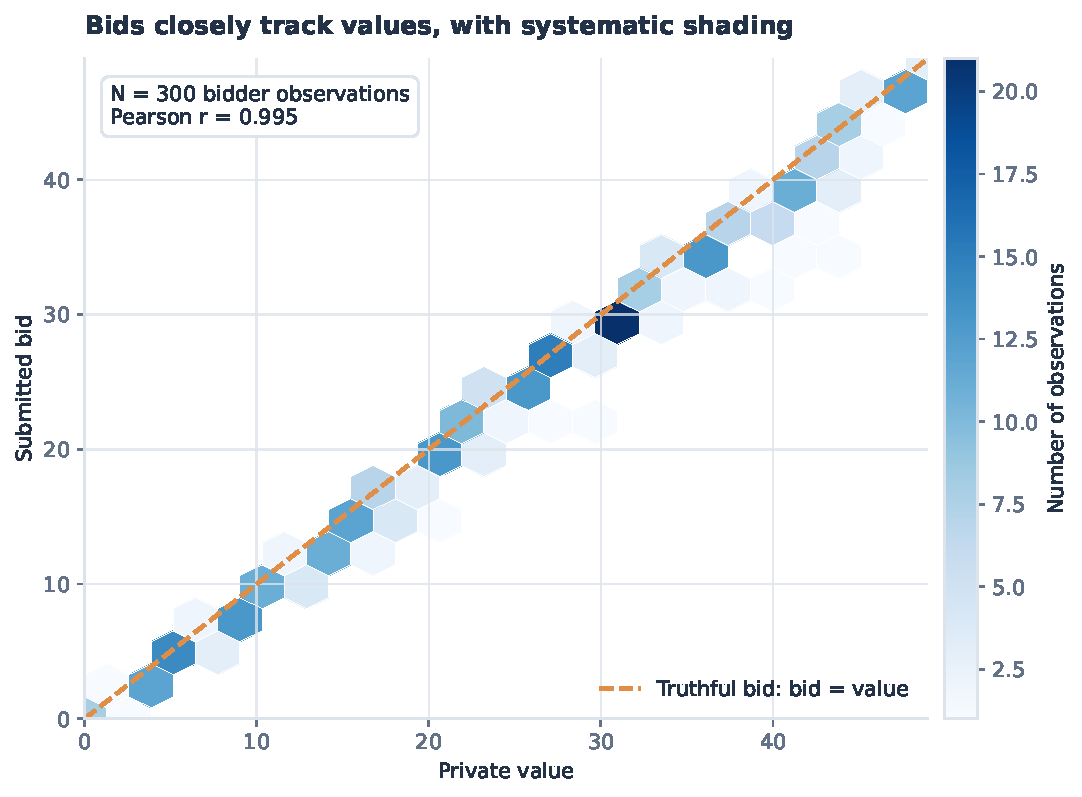
\includegraphics[width=0.82\textwidth]{figures/spsb_ipv_bid_value_density.pdf}
\caption{Bidder-level private values and submitted bids. Hexagon shading indicates the number of observations in each region; the dashed diagonal marks truthful bidding. All 300 observations are on or below the diagonal.}
\label{fig:bid-value}
\end{figure}

The next table groups observations into four value bands. Bid shading is defined as bid minus private value, so negative values indicate shading. The bands are descriptive bins, not estimated behavioral regimes.

\begin{center}
\begin{tabular}{lrrrr}
\toprule
Private-value band & Bidders & Mean value & Mean bid & Mean bid minus value \\
\midrule
0--12 & 68 & 6.338 & 5.719 & $-0.619$ \\
13--24 & 75 & 18.373 & 17.259 & $-1.115$ \\
25--36 & 85 & 30.365 & 29.324 & $-1.041$ \\
37--49 & 72 & 42.806 & 41.300 & $-1.506$ \\
\bottomrule
\end{tabular}
\end{center}

Average bids rise with value in every band, and average shading is largest in the top band. The single-run pattern is consistent with the plans' repeated emphasis on bidding below value to protect surplus. It does not establish that the plan question caused the shading: there is no paired run with the archived one-response prompt or with the plan question removed. Seat-level mean shading is similar (Andy: $-1.114$, Betty: $-1.080$, Charles: $-1.032$), which gives no strong descriptive sign of a seat-specific bidding difference in this sample. Figure~\ref{fig:shading} displays the full bidder-level distribution of bid minus value.

\begin{figure}[htbp]
\centering
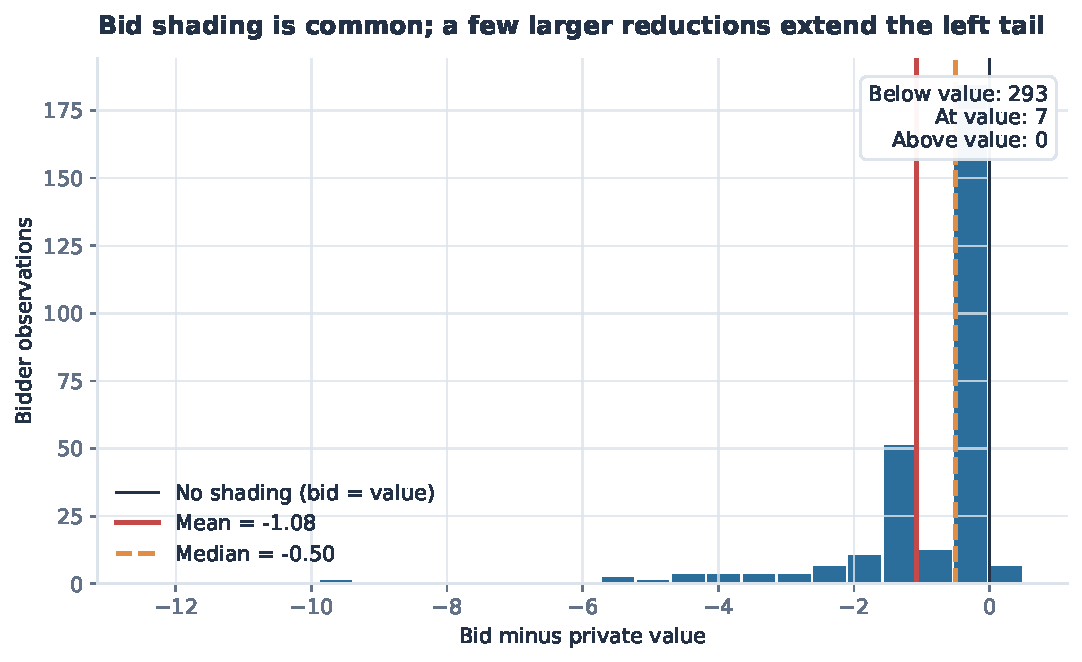
\includegraphics[width=0.82\textwidth]{figures/spsb_ipv_bid_shading_distribution.pdf}
\caption{Distribution of bid minus private value. Negative values indicate shading. The vertical lines show the sample mean and median; counts at the upper right show the number of bids below, at, and above value.}
\label{fig:shading}
\end{figure}

The auction outcomes show that shading did not often prevent the highest-value bidder from winning: 97 of 100 allocations are efficient. In the three exceptions, the winner's value is below the highest value by 5, 1, and 4 points, respectively, for 10 points of total realized allocation loss (0.10 per auction averaged over all 100). In repetition 6, Betty has value 30 but bids 21.5; Charles wins with value 25 after bidding 23.5. In repetition 15, Charles has the highest value (26) and bids 24.7, narrowly losing to Andy, whose value is 25 and bid is 24.9. In repetition 80, Andy has value 45 but bids 35.1; Betty wins with value 41 and bid 40.5. These cases illustrate the difference between a bid's private-value discipline and allocation efficiency: a bid can stay safely below value while being too conservative to win.

All 100 winning bidders earn positive modeled utility, with mean winner utility 12.288 and a median second-price payment of 24.75. Winner counts (33, 33, and 34) are close to balanced, as expected when seats are assigned symmetrically; the 100 auctions are too few to infer small seat effects. These outcome summaries describe the simulated auction rule and submitted bids. They are not evidence about human bidding, nor a treatment effect relative to the legacy experiment. Figure~\ref{fig:auction-outcomes} plots winner value against the highest available value and shows the distribution of winner utility.

\begin{figure}[htbp]
\centering
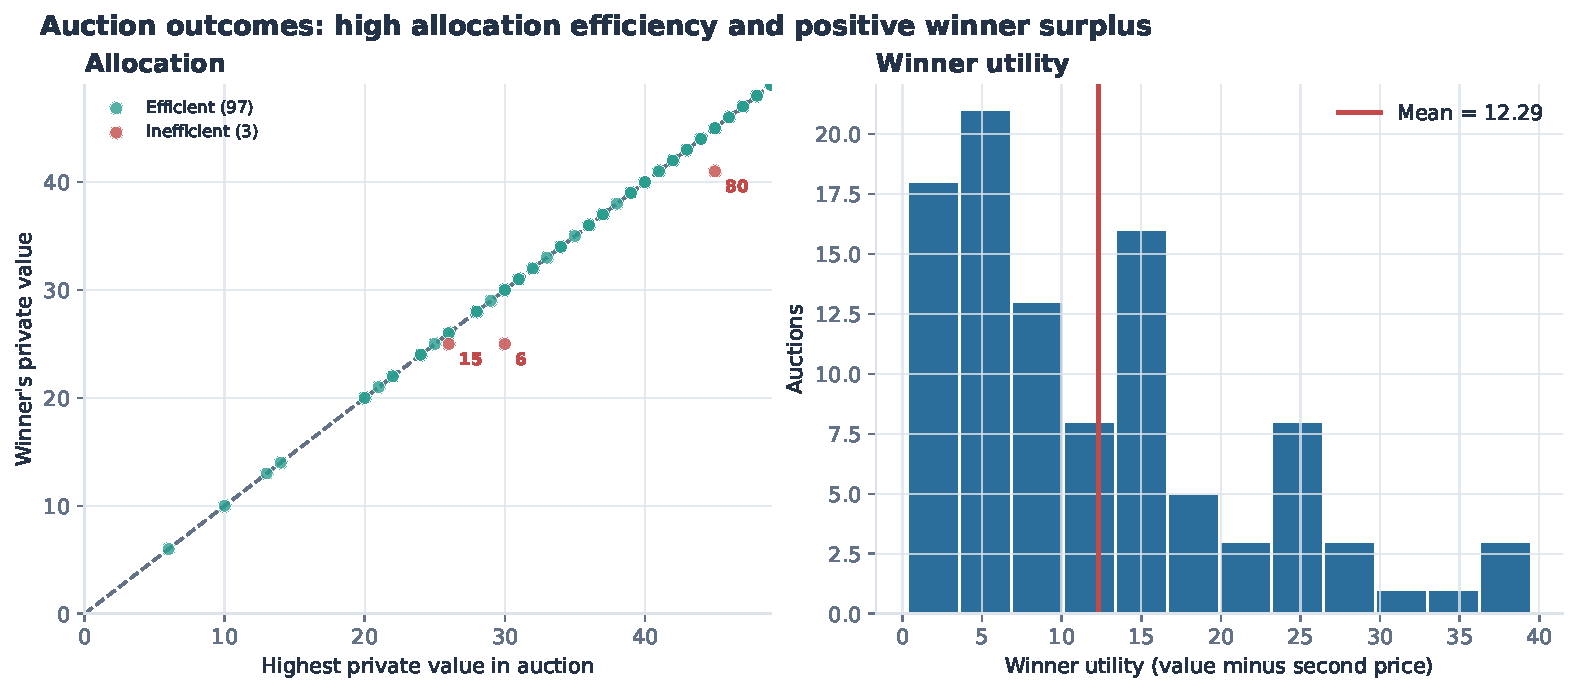
\includegraphics[width=0.98\textwidth]{figures/spsb_ipv_auction_outcomes.pdf}
\caption{Auction-level outcomes. Left: winner value against the highest private value in the auction; red points are inefficient allocations, labeled by repetition. Right: winner utility, defined as the winner's private value minus the second-highest bid.}
\label{fig:auction-outcomes}
\end{figure}

Raw EDSL output is saved at \texttt{edsl\_replication/runs/spsb\_ipv\_gpt4o\_100.json}. The derived bidder-level observations, auction-level outcomes, and summary are in \texttt{spsb\_ipv\_bidder\_results.csv}, \texttt{spsb\_ipv\_auction\_results.csv}, and \texttt{spsb\_ipv\_summary.json} in that directory. The exporter is \texttt{edsl\_replication/summarize\_spsb\_ipv.py}.

\clearpage
\appendix
\section{Treatment differences and implementation limits}

\begin{longtable}{p{0.24\linewidth}p{0.32\linewidth}p{0.34\linewidth}}
\toprule
Dimension & Legacy study & Current EDSL slice \\
\midrule
\endhead
Model response & One response with both plan and action tags & Separate plan and numerical bid questions \\
Bid validation & Nonnegative; configured increment checked; retries on invalid format & Numerical and nonnegative; increment and legacy retry policy not yet reproduced \\
Tie breaking & Random among tied highest bidders & Deterministic lower-seat priority \\
Settlement & Python post-processing in the auction class & Machine close expressions over stored bids \\
Visibility & Prompts assembled before a parallel survey call & Explicit read plus snapshot schedule; machine view seals bids \\
Run status & Archived study has recorded observations & 100 EDSL auctions completed; separate treatment \\
\bottomrule
\end{longtable}

The current code is an EDSL implementation prototype and the results are from a new treatment, not a result-reproducing treatment. To make it suitable for closer comparison, the next engineering pass should either implement the legacy one-response parse-and-retry path as a typed answer extraction step, or retain the split-question approach and label it as a new treatment. It should also add legacy tie selection and export adaptation for the existing analysis pipeline. A construction-only check preceded the full run; no separate scripted-answer test suite was run.

\section{Run environment and reproducibility}

The source cell, run status, and substantive results are in the main text. This appendix records the execution setup and initial provider troubleshooting for reproducibility.

\subsection{Run record}

\begin{center}
\begin{tabular}{ll}
\toprule
Item & Run record \\
\midrule
Completed bidder interviews & 300 / 300 \\
Settled auction scopes & 100 / 100 \\
Unfixed interview exceptions & 0 \\
Shared-state events & 700 \\
\bottomrule
\end{tabular}
\end{center}

The EDSL checkout at \texttt{~/tools/ep/edsl} is installed editable on \texttt{feature/shared-state-v0}, based at commit \texttt{1926cd297}. The branch subsequently renamed the Python exports \texttt{reduce\_} and \texttt{set\_} to \texttt{reduce} and \texttt{assign}; the reducer expression and serialized set effect are unchanged. The auction port and examples in this note use the current names. The 100-auction observations were collected before that API-only rename; they do not depend on the Python spelling of these constructors. The first provider attempt in the sandbox timed out; the successful run used approved outbound access to OpenAI. Model construction selected the \texttt{openai} service because the active profile's cached model catalogue did not list GPT-4o. The key was loaded from the project \texttt{.env}; its value is intentionally not reproduced here.

The job was constructed and run by the local EDSL Python process. For this YAML, \texttt{Model("gpt-4o", service\_name="openai")} selected the OpenAI provider. EDSL loaded \texttt{OPENAI\_API\_KEY} from the project \texttt{.env}. The EDSL runner and SQLite shared-state backend ran locally; model inference was performed by OpenAI. This execution uses a provider API key and does not require a local model server.

The split question protocol generated at least 600 model responses (one plan and one bid response for each bidder). The saved Results object contains the answer values and plan text along with the shared-state event history. The exact command is shown in the main-text run section.

\section{Source map}

\begin{itemize}
  \item Auction port: \texttt{edsl\_replication/spsb\_ipv\_shared\_state.py}
  \item Port limitations and invocation: \texttt{edsl\_replication/README.md}
  \item Raw run and derived outputs: \texttt{edsl\_replication/runs/spsb\_ipv\_gpt4o\_100.json}, \texttt{spsb\_ipv\_bidder\_results.csv}, \texttt{spsb\_ipv\_auction\_results.csv}, and \texttt{spsb\_ipv\_summary.json}
  \item Figure generator and editable assets: \texttt{edsl\_replication/plot\_spsb\_ipv.py} and \texttt{writeup/figures/} (PDF and PNG versions)
  \item Machine diagram generator: \texttt{edsl\_replication/render\_spsb\_ipv\_machine.py}; rendered by the EDSL \texttt{Machine.show\_diagram()} method
  \item Shared-state model and scoped handles: \texttt{edsl/sharedstate/model.py}
  \item DSL and interpreter: \texttt{edsl/sharedstate/dsl.py}, \texttt{edsl/sharedstate/dsl\_runtime.py}
  \item SQLite event backend: \texttt{edsl/sharedstate/backend.py}
  \item Runner read/write/finalization integration: \texttt{edsl/runner/service.py}
  \item Schedule declaration and validation: \texttt{edsl/jobs/interview\_schedule.py}
  \item Experimental shared-state contract: \texttt{docs/shared\_state.md} in the EDSL checkout.
\end{itemize}

\end{document}
